\chapter{Návrh}
\label{sec:de}

\section{Architektura MVC}

\begin{figure}[h!]
    \centering
    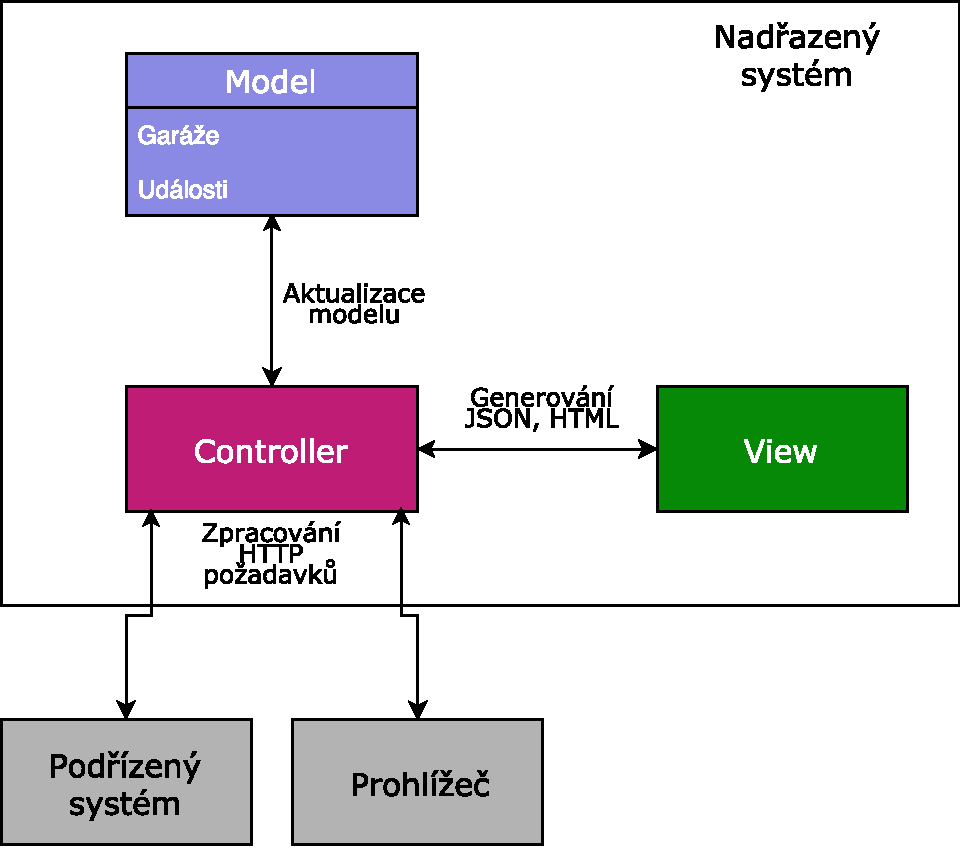
\includegraphics[width=0.7\textwidth]{images/mvc.pdf}
    \caption{Struktura MVC aplikace}
    \label{fig:mvc}
\end{figure}

???

controller -- api, zpracovavani http requestu

view -- webova stranka

model -- vyhodnocovani a logovani udalost, stavu garazi

???

viz \url{https://www.digitalocean.com/community/tutorials/how-to-structure-large-flask-applications#working-with-modules-and-blueprints-(components)}

\section{Model}

pouziti sqlalchemy -- to resit az v~implementaci

\subsection{Garáž}

\subsubsection{Stav garáže}

\subsection{Událost}

\subsubsection{Vyhodnocení události}

\section{Controller}

Flask API

\section{View}

\section{Autentizace}

\subsection{Autentizace uživatele}

\subsection{Autentizace podřízeného systému}

\subsubsection{Registrační mód}

